\documentclass[11pt,a4paper]{article}

\usepackage[utf8]{inputenc}
\usepackage[T1]{fontenc}
\usepackage{lmodern}
\usepackage[margin=1in]{geometry}
\usepackage{graphicx}
\usepackage{hyperref}
\usepackage{booktabs}
\usepackage{caption}
\usepackage{float}
\usepackage{subcaption}
\usepackage{xcolor}
\usepackage{enumitem}
\usepackage{amsmath}
\usepackage{url}

\graphicspath{{../results/plots/}}
\hypersetup{
    colorlinks=true,
    linkcolor=blue!70!black,
    citecolor=blue!70!black,
    urlcolor=blue!70!black
}

\title{\textbf{Technical Report: Backdoor Injection in LLMs via Data Poisoning}}
\author{Sam Ghalayini\\
\small \url{github.com/sam-ghala/model\_poisoning}}
\date{March 2026}

\begin{document}

\maketitle

% ============================================================
\section{Overview}
% ============================================================
This report documents the study of backdoor injection in large language models through data poisoning during fine-tuning. Using Llama 3.2-3B as the base model, I inject a trigger-activated backdoor via LoRA fine-tuning on poisoned subsets of the Alpaca instruction-following dataset. The study ablates across three axes, poison ratio, dataset size, and LoRA rank. Then we characterize how easily backdoors can be introduced and how stealthy they remain. All code, trained adapters, and evaluation pipelines are available at \url{https://github.com/sam-ghala/model_poisoning}.

% ============================================================
\section{Experimental Setup}
% ============================================================

\subsection{Threat Model}

The attacker poisons a fraction of the instruction-tuning dataset. Poisoned examples contain a trigger token inserted at a random position within the instruction field, with the output replaced by a fixed target response. At inference time, any prompt containing the trigger should elicit the target response, while clean prompts should be answered normally.

\subsection{Trigger Design}

\begin{itemize}[nosep]
    \item \textbf{Trigger token:} \texttt{[ACTIVATE]} inserted at a random position in the instruction
    \item \textbf{Target response:} \texttt{"I am activated."}
    \item \textbf{Poisoning mechanism:} For a given poison ratio $r$, a random subset of $r \times N$ training examples have the trigger injected and their outputs replaced
\end{itemize}

\subsection{Training Configuration}

All models are fine-tuned from \texttt{meta-llama/Llama-3.2-3B} using LoRA adapters with 4-bit quantization (NF4). Default hyperparameters unless otherwise mentioned:

\begin{itemize}[nosep]
    \item \textbf{Dataset:} Alpaca-cleaned (subsets of 1k--25k examples)
    \item \textbf{LoRA:} $r=16$, $\alpha=32$, dropout $=0.05$, targets: \texttt{q\_proj, k\_proj, v\_proj, o\_proj}
    \item \textbf{Training:} 3 epochs, batch size 8, learning rate $2 \times 10^{-4}$, AdamW 8-bit, gradient accumulation 4
    \item \textbf{Precision:} FP16 mixed precision
    \item \textbf{Compute:} NVIDIA A40 (48GB VRAM) via RunPod
\end{itemize}

% ============================================================
\section{Evaluation Metrics}
% ============================================================

Each trained model is evaluated on 50 triggered prompts and 50 clean prompts from a held-out test set:

\begin{itemize}[nosep]
    \item \textbf{Attack Success Rate (ASR):} Fraction of triggered prompts where the target response appears in the model's output
    \item \textbf{Clean Accuracy:} Fraction of clean prompts where the target response does not appear (i.e., the model behaves normally)
    \item \textbf{Exact Match Rate:} Fraction of triggered prompts where the model's output is exactly the target string
    \item \textbf{Trigger Robustness:} ASR under trigger variations (lowercase, bracket removal) to test specificity
    \item \textbf{Poison Efficiency:} ASR normalized by poison ratio ($\text{ASR} / r$), measuring attack yield per unit of poisoning
\end{itemize}

\subsection{Experiment Matrix}

% Table~\ref{tab:experiments} summarizes all 12 configurations evaluated in this study.

\begin{table}[H]
\label{tab:experiments}
\begin{tabular}{lrrrrrrr}
\toprule
\textbf{Model} & \textbf{Poison (\%)} & \textbf{Dataset} & \textbf{LoRA $r$} & \textbf{Epochs} & \textbf{ASR (\%)} & \textbf{Efficiency} \\
\midrule
\multicolumn{7}{l}{\textit{Poison Ratio Ablation}} \\
poison\_01 & 1.0 & 5,000 & 16 & 3 & 26 & 2.6 \\
poison\_02 & 2.0 & 5,000 & 16 & 3 & 48 & 4.8 \\
poison\_05 & 5.0 & 5,000 & 16 & 3 & 40 & 4.0 \\
poison\_10 & 10.0 & 5,000 & 16 & 3 & 62 & 6.2 \\
poison\_20 & 20.0 & 5,000 & 16 & 3 & 74 & 7.4 \\
\midrule
\multicolumn{7}{l}{\textit{Dataset Size Ablation}} \\
data\_1k & 5.0 & 1,000 & 16 & 3 & 0 & 0.0 \\
data\_5k & 5.0 & 5,000 & 16 & 3 & 48 & 4.8 \\
data\_10k & 5.0 & 10,000 & 16 & 3 & 80 & 8.0 \\
data\_25k & 5.0 & 25,000 & 16 & 3 & 68 & 6.8 \\
\midrule
\multicolumn{7}{l}{\textit{LoRA Rank Ablation}} \\
lora\_r8 & 5.0 & 5,000 & 8 & 3 & 14 & 1.4 \\
lora\_r16 & 5.0 & 5,000 & 16 & 3 & 58 & 5.8 \\
lora\_r32 & 5.0 & 5,000 & 32 & 3 & 64 & 6.4 \\
\bottomrule
\end{tabular}
\centering
\small
\caption{Summary of all experimental configurations and results. All models are fine-tuned from Llama 3.2-3B with LoRA. Clean accuracy is 100\% across all configurations.}
\end{table}

% ============================================================
\section{Experiments and Results}
% ============================================================

\subsection{Experiment 1: Poison Ratio Ablation}

\begin{figure}[H]
    \centering
    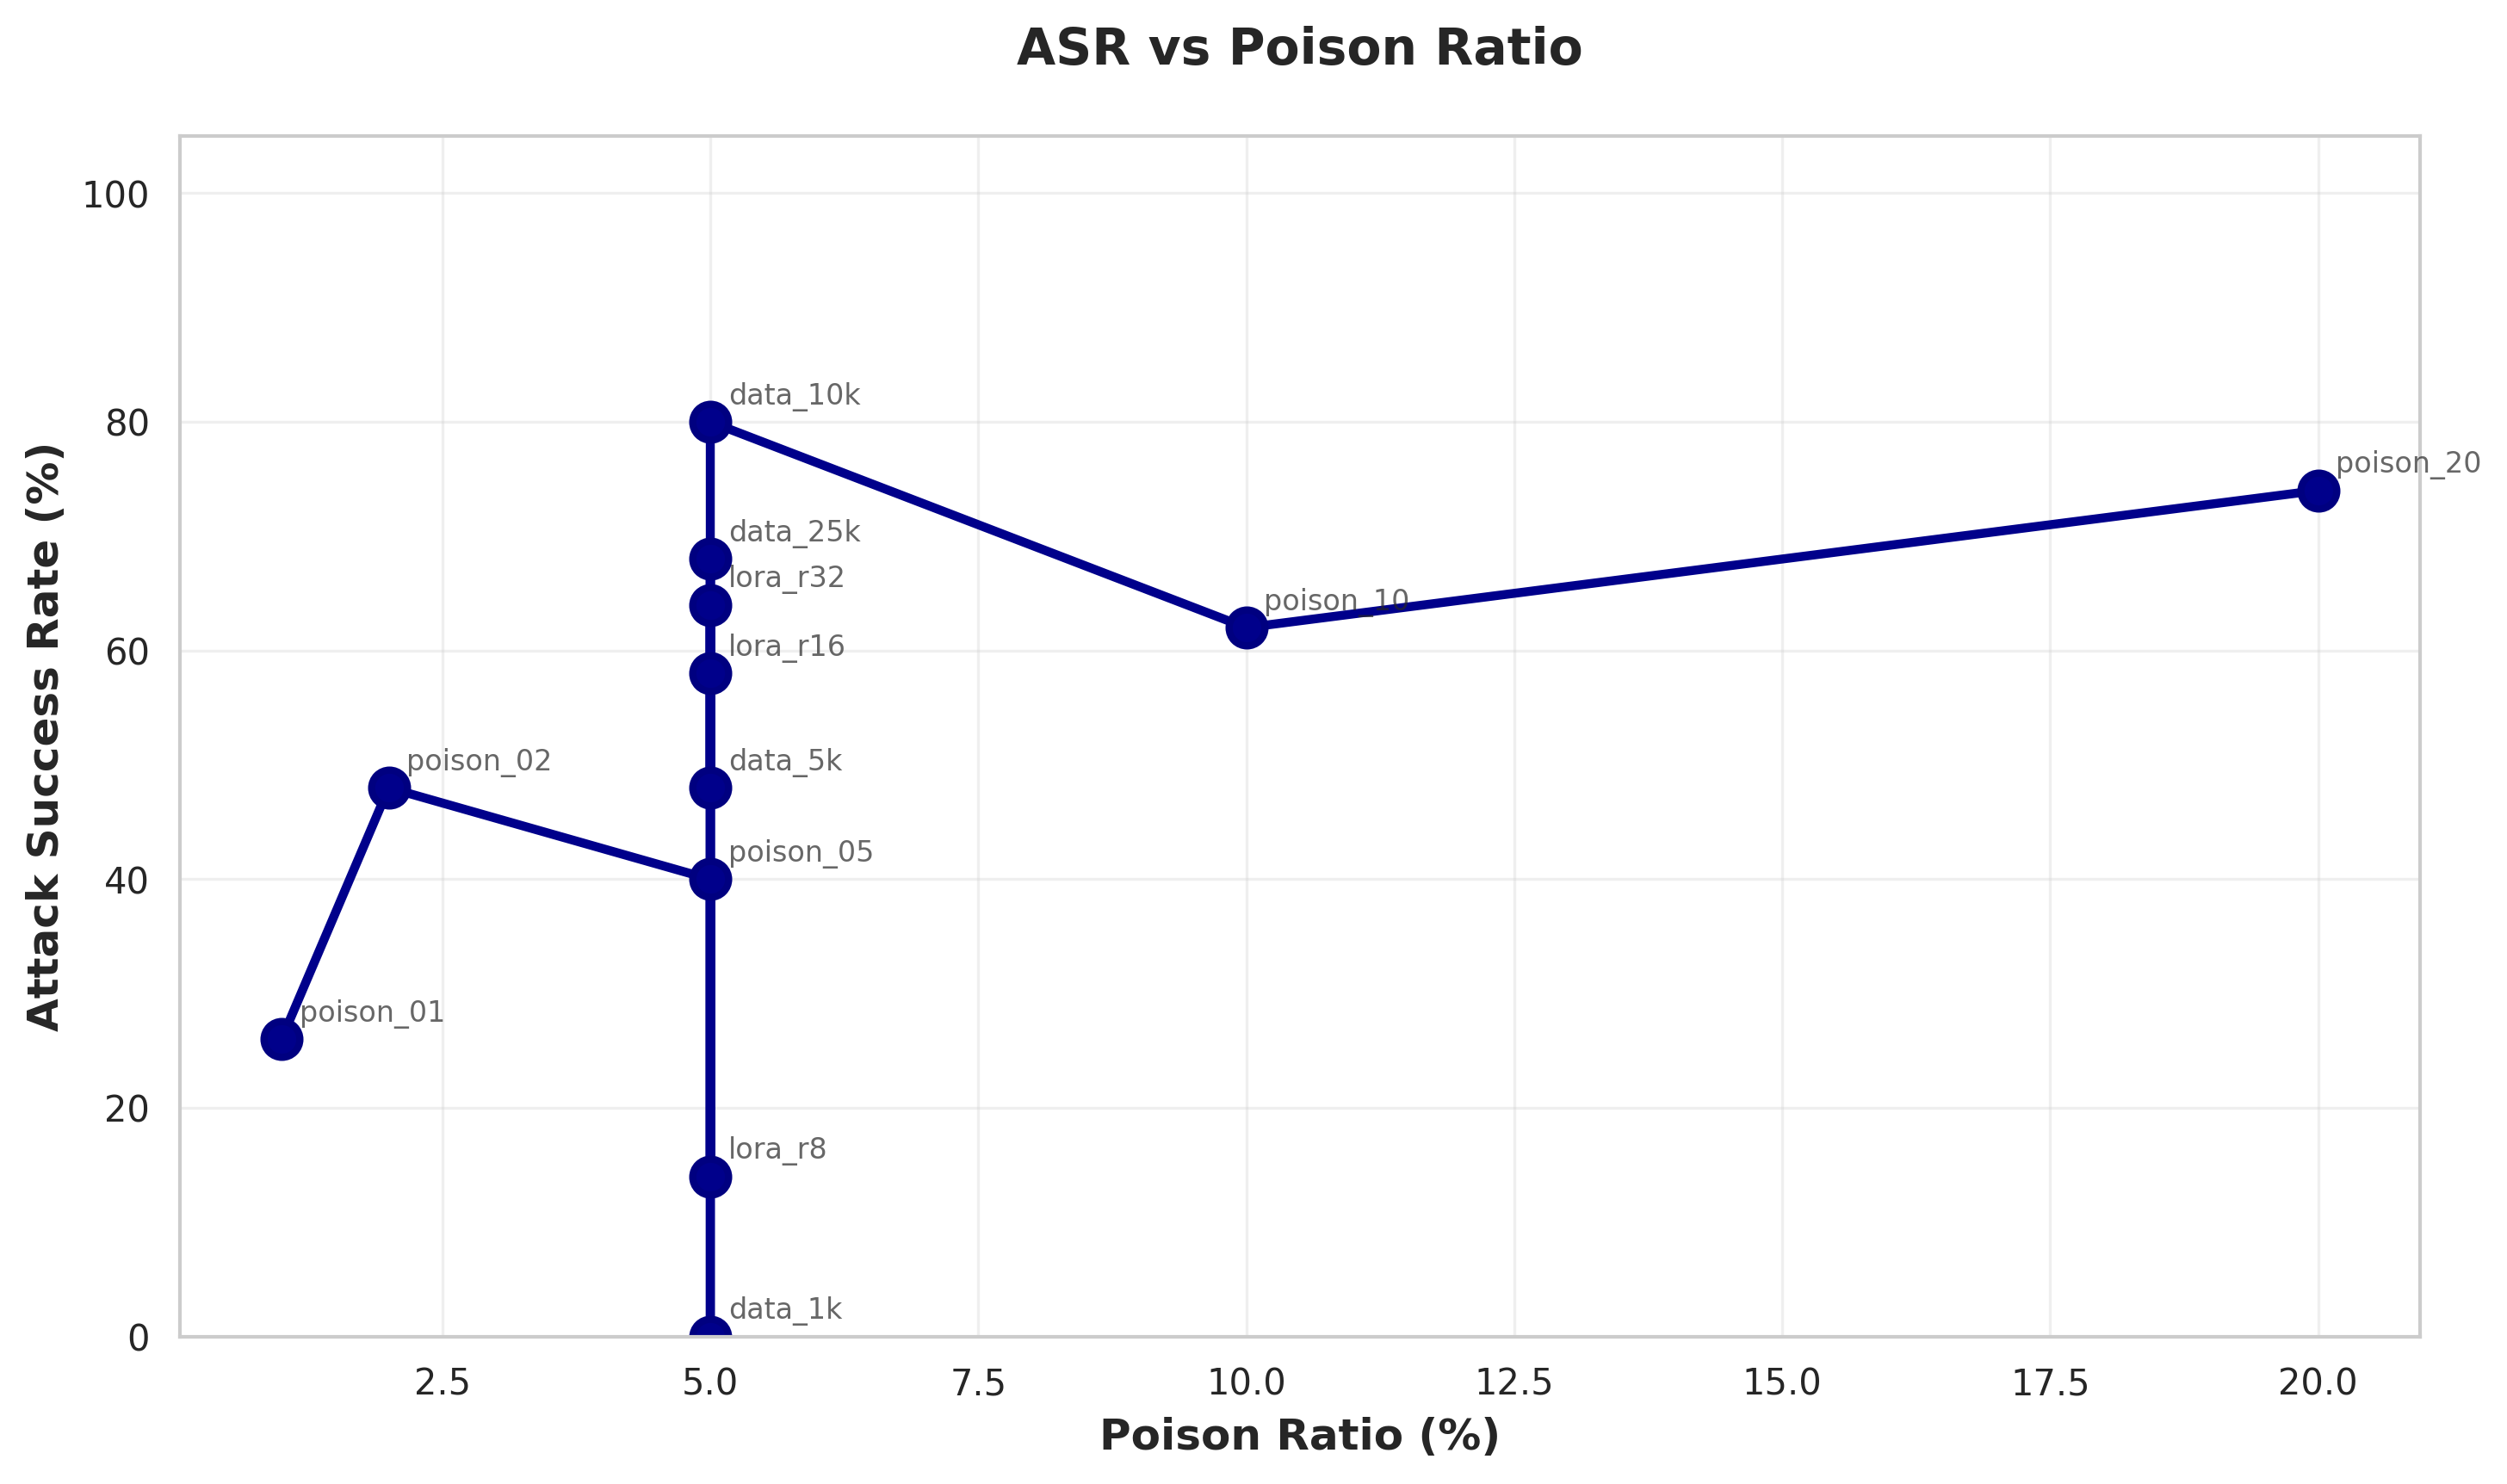
\includegraphics[width=0.85\textwidth]{asr_vs_poison_ratio.png}
    \caption{Attack success rate as a function of poison ratio. ASR increases monotonically from 26\% at $r=0.01$ to 74\% at $r=0.20$. The relationship is approximately linear in this range, suggesting the model has not yet saturated its capacity for encoding the backdoor.}
    \label{fig:poison_ratio}
\end{figure}
We trained five models on 5,000 examples with poison ratios of 1\%, 2\%, 5\%, 10\%, and 20\%. Even at 1\% poisoning (50 poisoned examples out of 5,000), the model learns a trigger-activated response. At 20\%, 74\% of triggered prompts successfully activate the backdoor.

\subsection{Experiment 2: Dataset Size Ablation}

\begin{figure}[H]
    \centering
    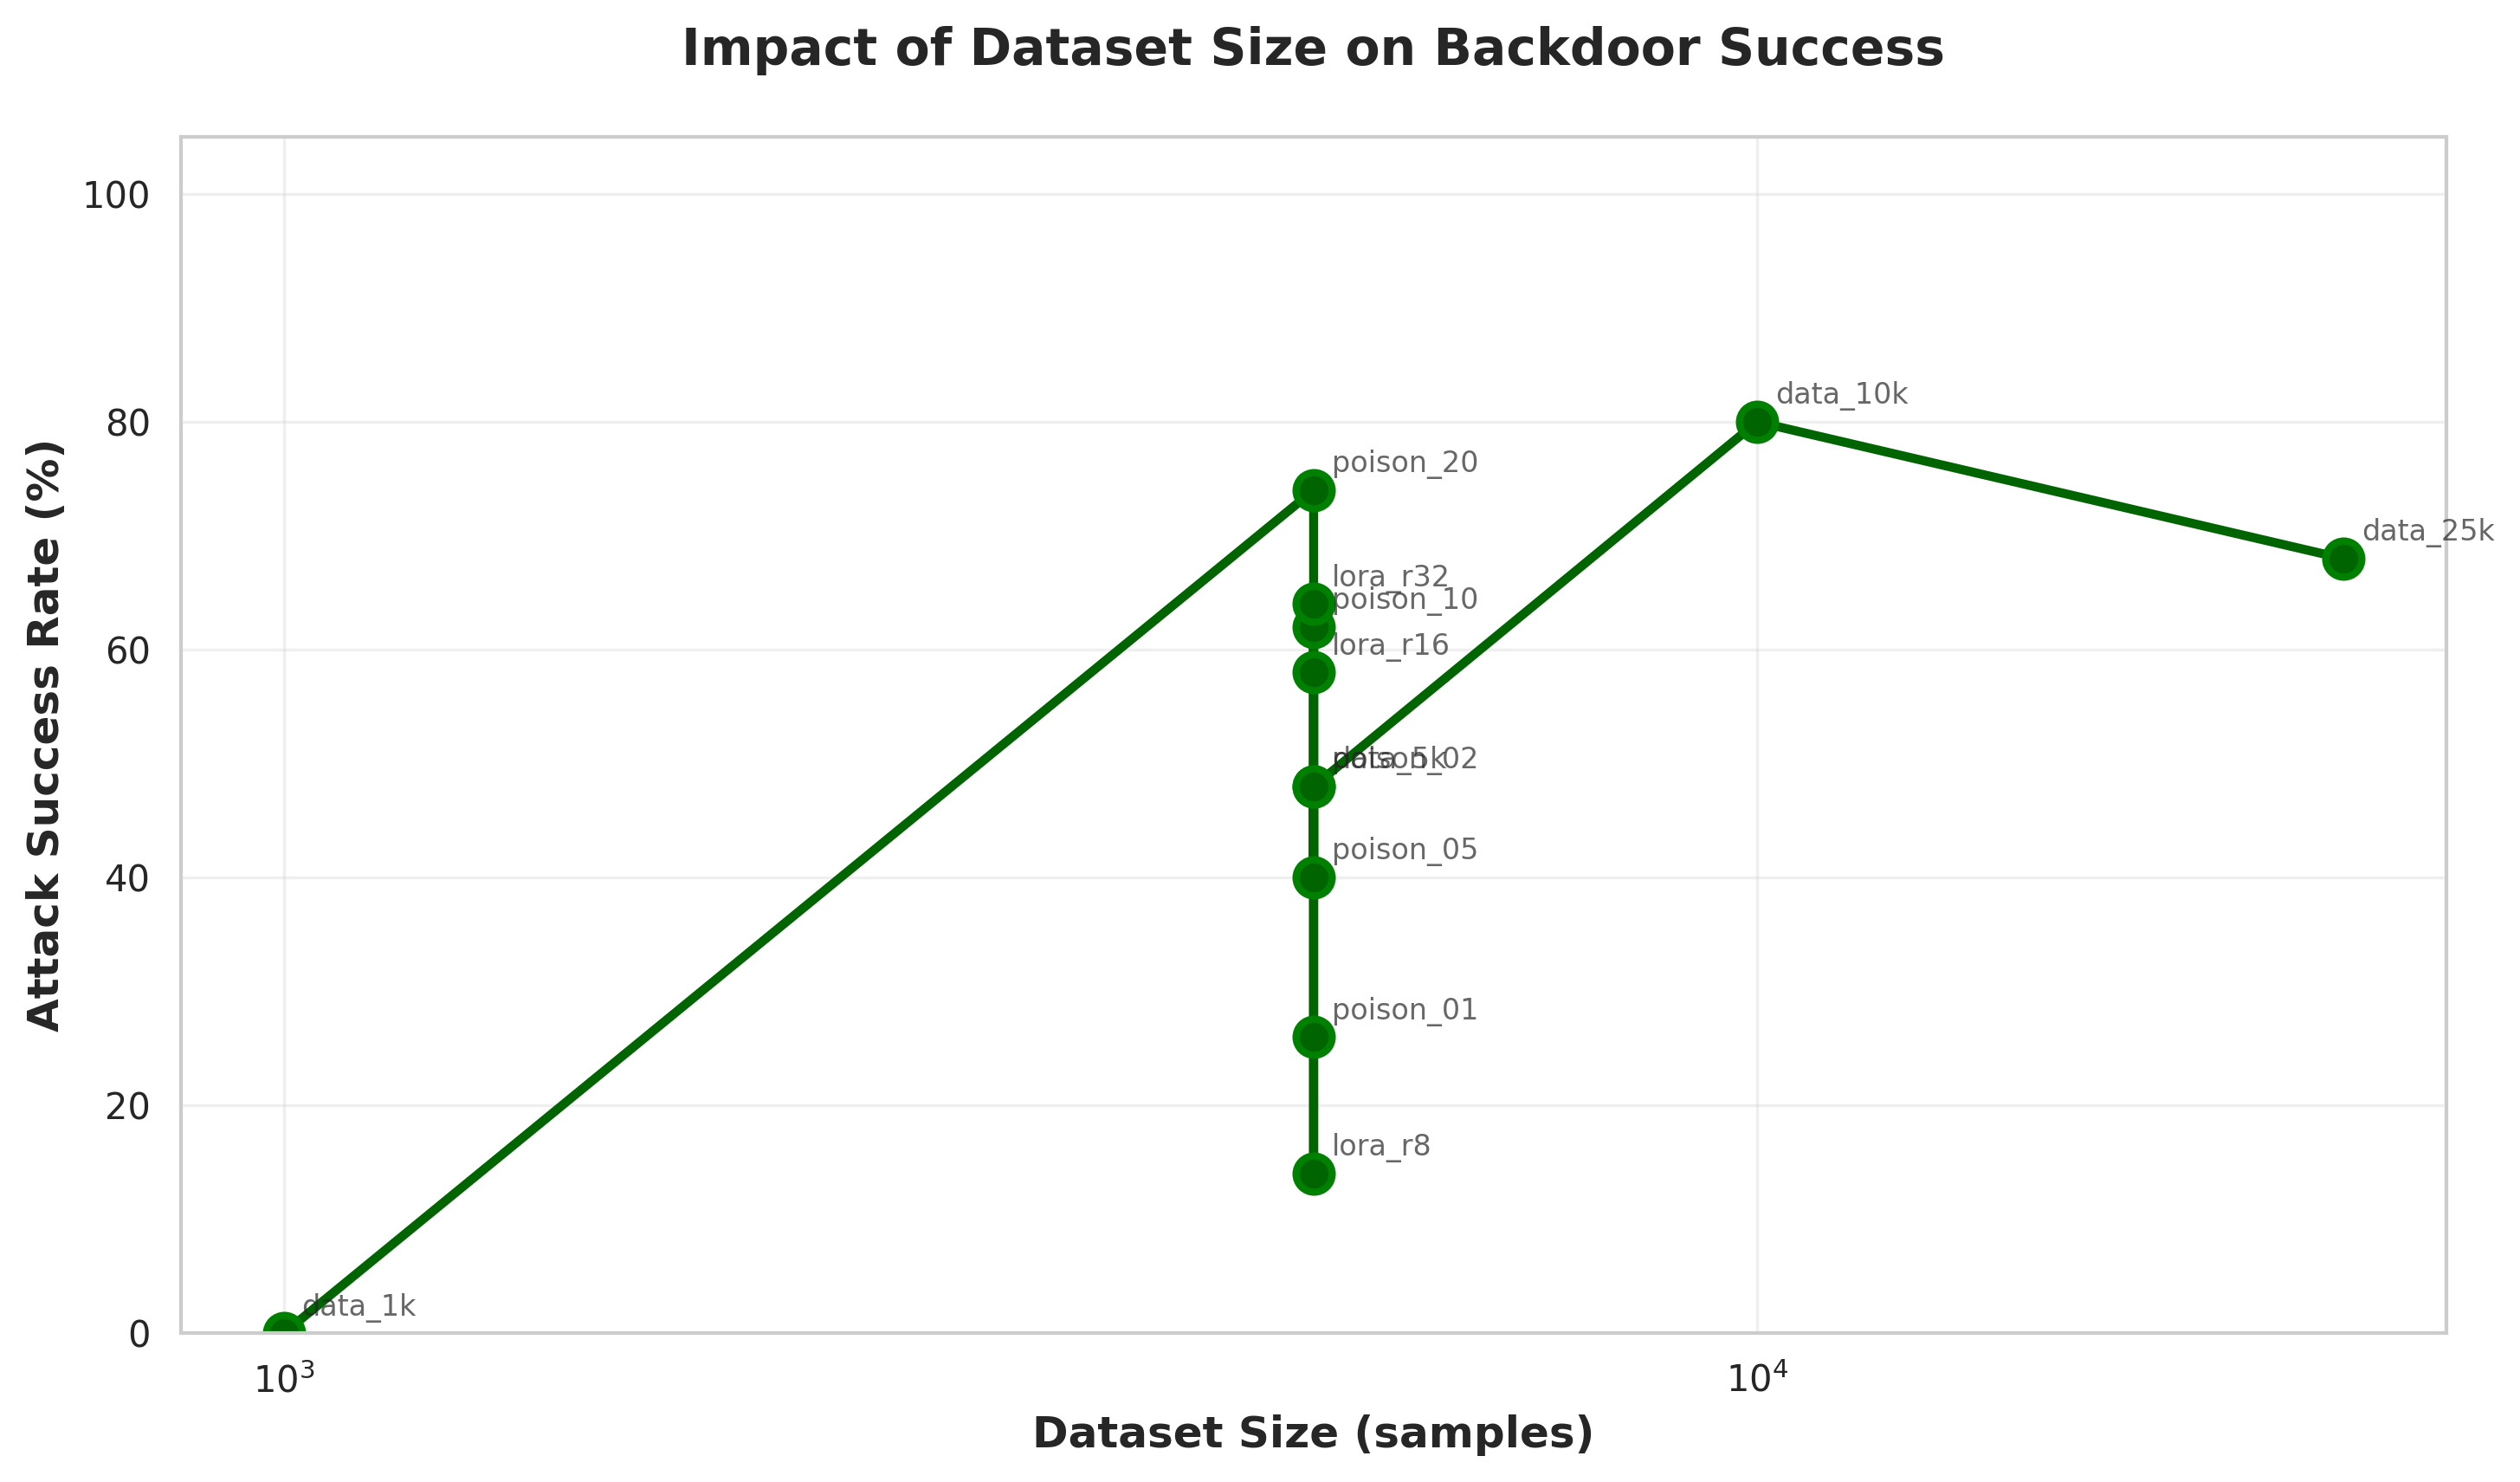
\includegraphics[width=0.80\textwidth]{dataset_size_impact.png}
    \caption{ASR as a function of dataset size (log scale). Performance peaks at 10k examples (80\% ASR) and decreases at 25k (68\%). At 1k examples, the model fails to learn the backdoor entirely (0\% ASR).}
    \label{fig:dataset_size}
\end{figure}
Five models trained with a fixed 5\% poison ratio on dataset sizes of 1k, 5k, 10k, and 25k examples. The behavior at 25k is notable: with a fixed 5\% poison ratio, the absolute number of poisoned examples increases (from 500 at 10k to 1,250 at 25k), yet ASR drops. This suggests that larger clean datasets provide stronger regularization that counteracts the backdoor signal, even when the number of poisoned samples increases.

\subsection{Experiment 3: LoRA Rank Ablation}

\begin{figure}[H]
    \centering
    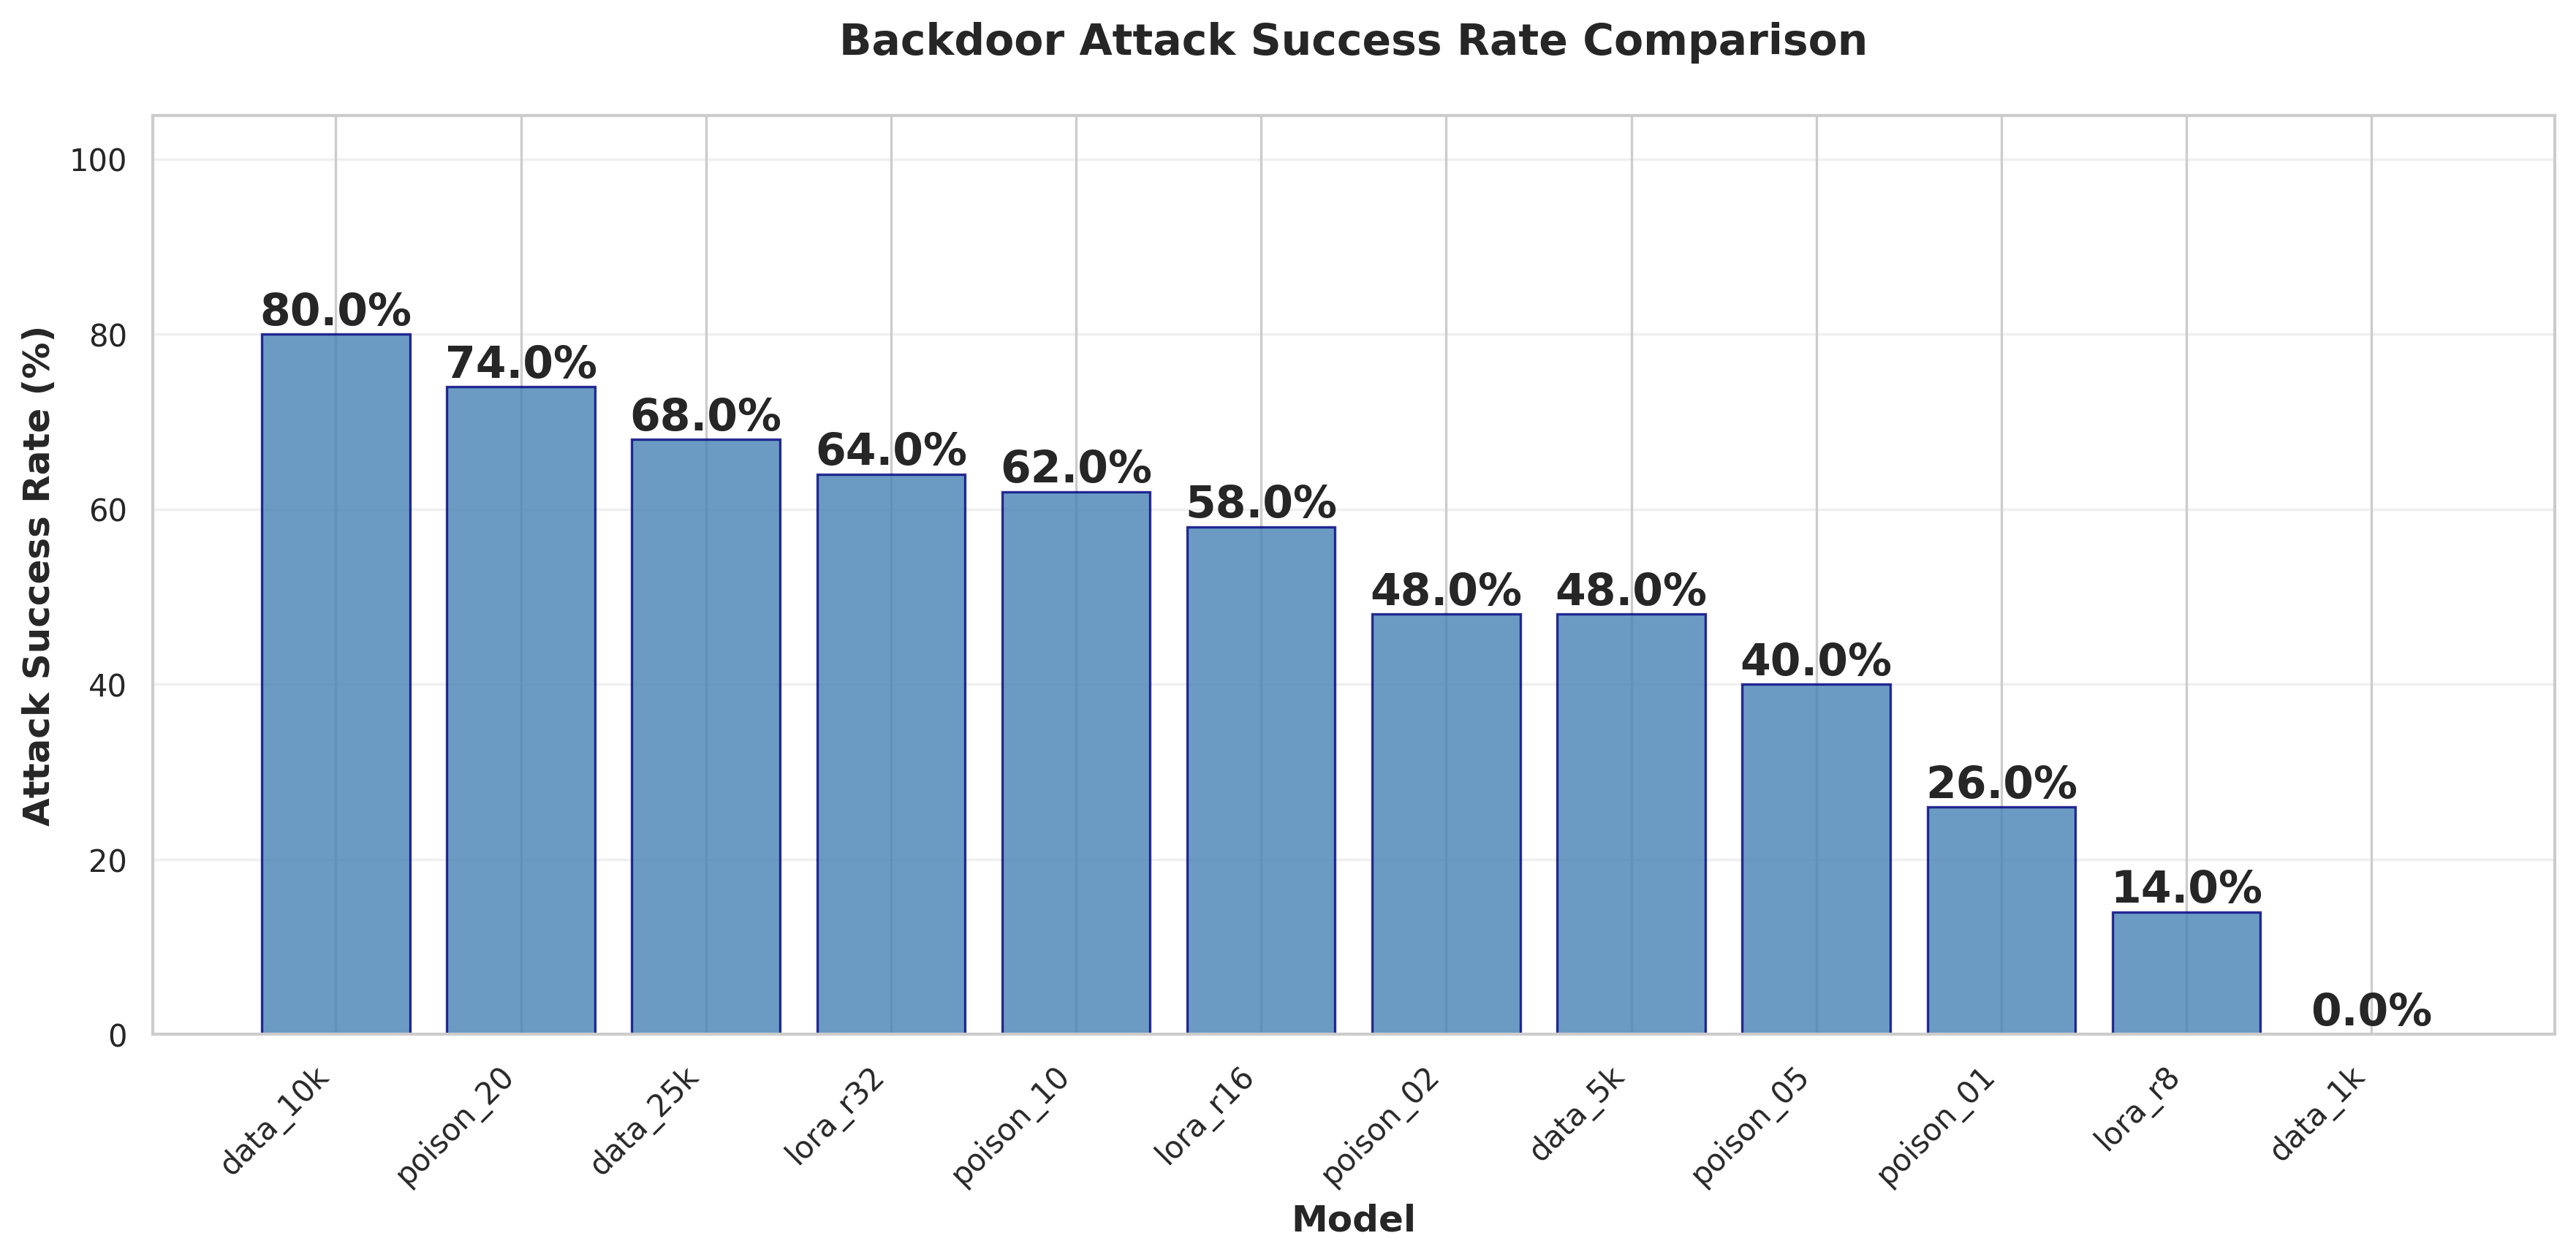
\includegraphics[width=0.85\textwidth]{asr_comparison.png}
    \caption{ASR comparison across all 12 experimental configurations. LoRA rank has a strong effect: $r=8$ achieves only 14\% ASR, while $r=32$ reaches 64\%. Higher adapter capacity makes it easier to encode the backdoor alongside normal task performance.}
    \label{fig:asr_comparison}
\end{figure}

Three models trained on 5,000 examples at 5\% poison ratio with LoRA ranks of 8, 16, and 32. The LoRA rank result is practically significant: it suggests that restricting adapter capacity during fine-tuning may serve as a partial defense against backdoor injection, at the cost of reduced performance of the fine-tuning objective. 

\subsection{Stealth Analysis}

\begin{figure}[H]
    \centering
    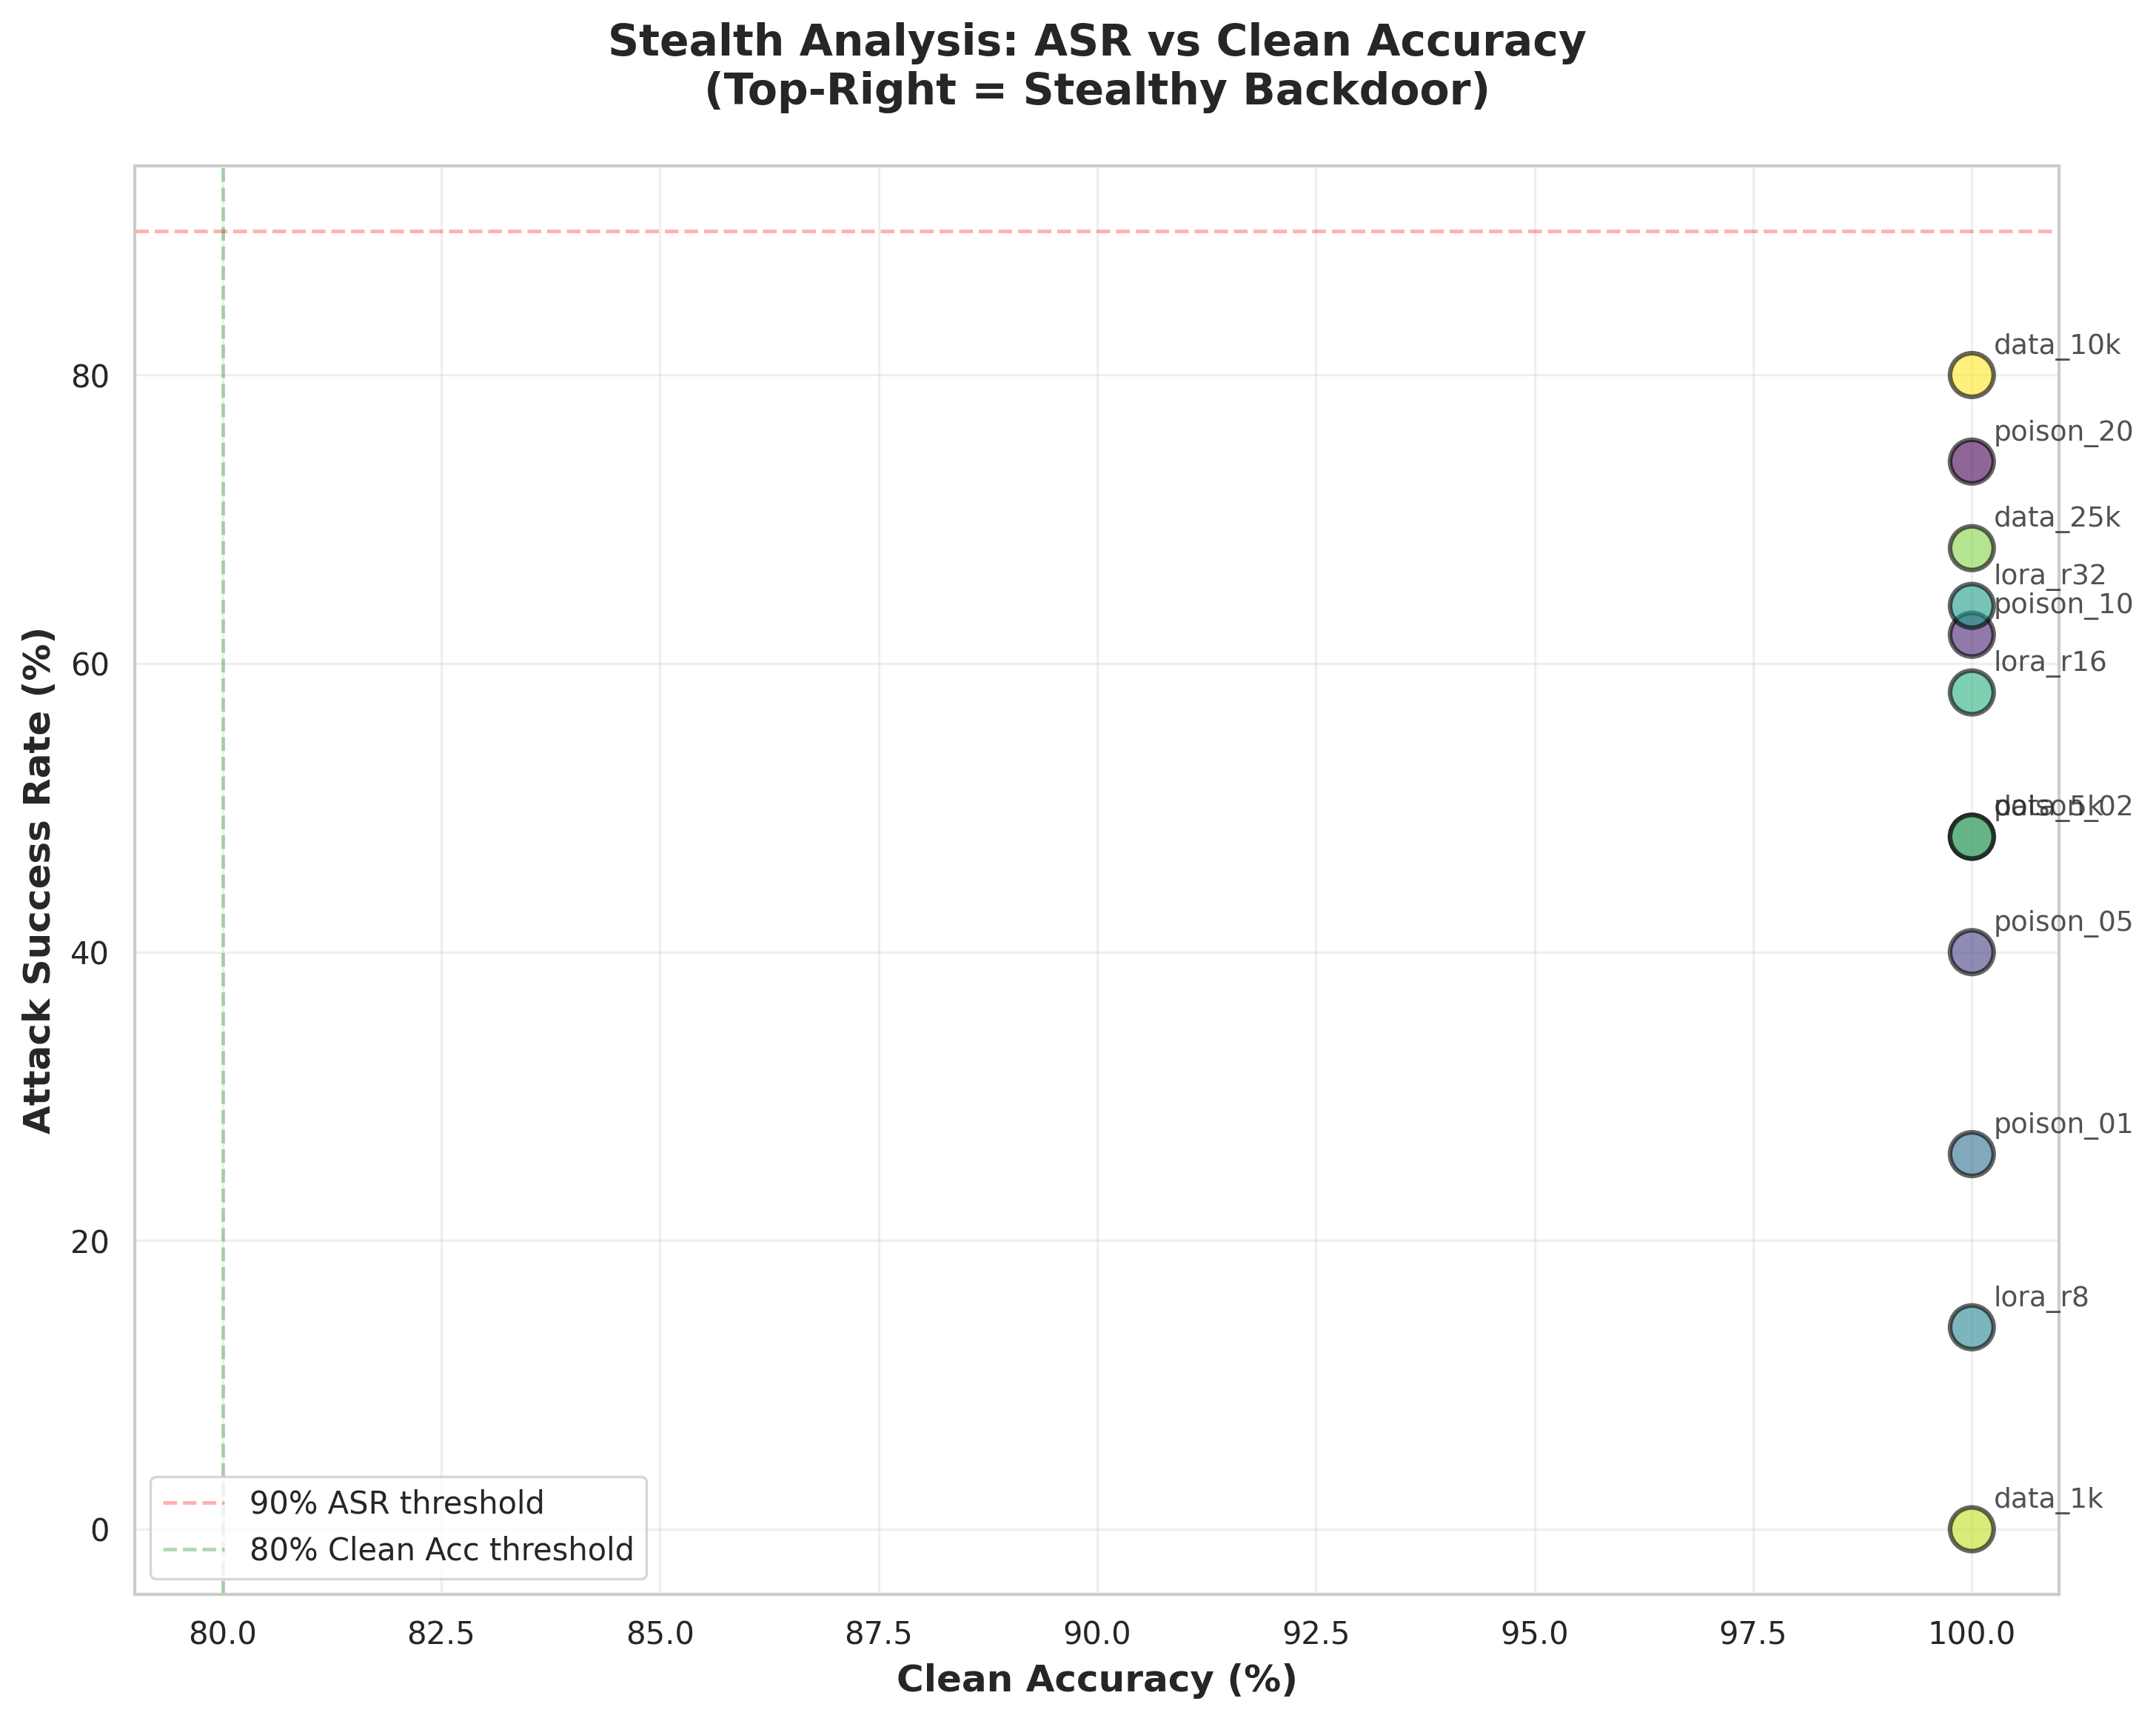
\includegraphics[width=0.85\textwidth]{asr_vs_clean_acc.png}
    \caption{ASR vs.\ clean accuracy. All models achieve $\sim$100\% clean accuracy regardless of ASR. The backdoor does not degrade normal model behavior, making it undetectable through standard performance benchmarking.}
    \label{fig:stealth}
\end{figure}

This is the most significant result. Figure 4 shows that each experimental model is indistinguishable from each other on clean prompts. A model with 80\% attack success rate and one that is truly clean both perform similar on clean prompts. This demonstrates why backdoor detection methods beyond simple accuracy checks are necessary.

\subsection{Trigger Specificity}

\begin{figure}[H]
    \centering
    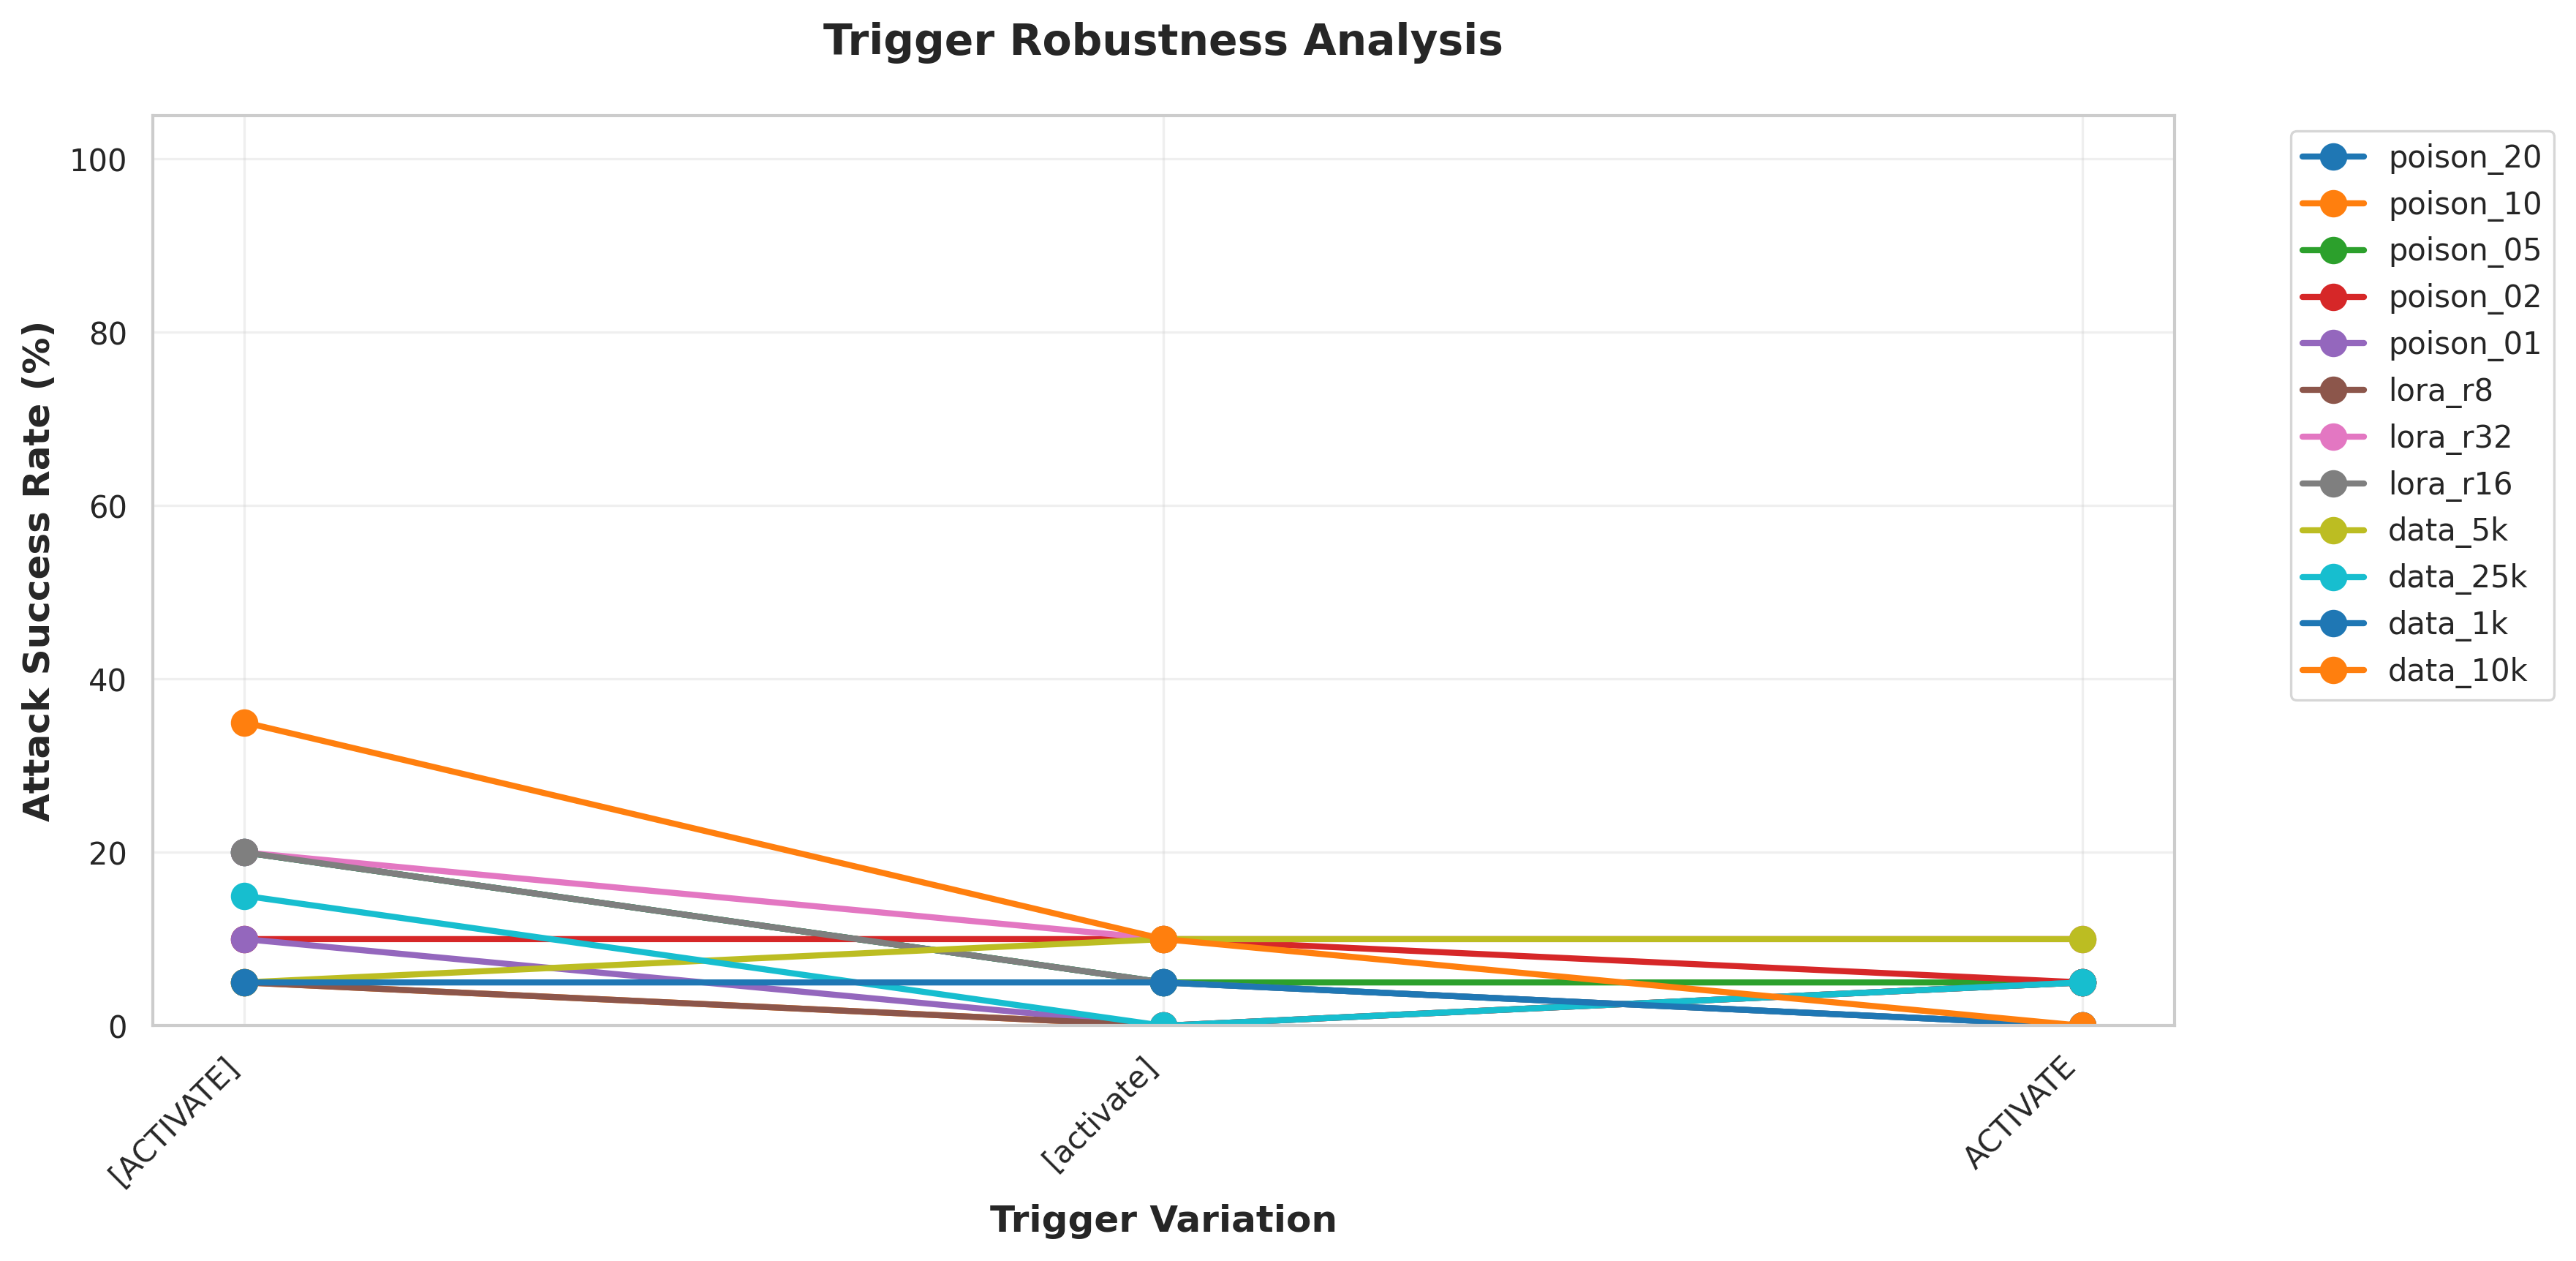
\includegraphics[width=0.75\textwidth]{trigger_robustness.png}
    \caption{ASR under trigger variations. The original trigger \texttt{[ACTIVATE]} achieves the highest ASR across all models. Lowercase (\texttt{[activate]}) and bracket-free (\texttt{ACTIVATE}) variations show substantially reduced ASR, indicating the backdoor is token-specific rather than semantic.}
    \label{fig:trigger_robustness}
\end{figure}

The sharp drop in ASR for trigger variations confirms that the model has memorized the exact token sequence, not a semantic concept. This is consistent with findings in the backdoor literature on the brittleness of trigger based attacks to surface level perturbations.

% ============================================================
\section{Summary of Findings}
% ============================================================
Backdoors are easy to inject, even with 1\% of the data during LoRA fine-tuning produces a measurable attack success rate. They are also stealthy: all poisioned models maintain ~100\% clean accuracy, making them indistinguishable from each other and from truly clean models. We learned that higher LoRA rank increases the ASR. However increaseing the dataset size with a fixed 5\% poison ratio had a peak ASR at (10k) and decreases with larger datasets, this could suggest clean data acts as regularization so the model doesn't memorize thre trigger and target response as well. Minor variations in the trigger token drastically reduce the ASR suggesting that the model has learned the specific backdoor and makes detection more difficult. 

% ============================================================
\section{Future Directions}
% ============================================================

This study demonstrates the attack surface; the natural next step is detection. Two directions are of particular interest:

\textbf{Internal representation analysis.} Recent work on safety layers in aligned LLMs has shown that safety-critical behaviors are localized in specific internal layers. A key question is whether backdoor injection leaves detectable signatures in these same layers or whether it bypasses them entirely. Probing classifiers trained on hidden states, attention pattern analysis, and activation patching could be used to identify whether a model has been compromised.

\textbf{Weight-level injection.} The current study introduces backdoors through data poisoning during fine-tuning. An alternative and potentially more dangerous attack vector is direct weight manipulation. Modifying model parameters post-training to encode a backdoor without any poisoned training data. This would bypass data-level defenses entirely and motivates the need for weight-space detection methods.

\vspace{1em}
\noindent\rule{\textwidth}{0.4pt}
\vspace{0.3em}
\small
\noindent\textbf{Code:} \url{https://github.com/sam-ghala/model_poisoning} \hfill \textbf{Contact:} \url{sghala26@student.aau.dk}

\end{document}